\section{NVIDIA's architectures and compiler flow}

This section provides background on basic GPU architecture terminology
and the NVIDIA GPU compilation flow.  Some of the examples later in
this guide require a baseline level of knowledge about GPU
architectures. 

\subsection{Architecture Terminology}

GPU programming models allow the creation of thousands of threads that
each execute the same code. Threads are grouped into 32-element
vectors called \emph{warps} to improve efficiency. The threads in each
warp execute in a SIMT (\emph{single instruction, multiple thread})
fashion, all fetching from a single Program Counter (PC) in the
absence of control flow.  Many warps are then assigned to execute
concurrently on a single GPU core, or \emph{streaming multiprocessor}
(SM). A GPU consists of multiple such SM building blocks along with a
memory hierarchy including SM-local scratchpad memories and L1 caches,
a shared L2 cache, and multiple memory controllers. Different GPUs
deploy differing numbers of SMs.

\subsection{GPU Software Stack}

Historically, NVIDIA has referred to units of code that run on the GPU
as \emph{shaders}.  There are several broad categories of shaders,
including DirectX shaders, OpenGL shaders, and compute shaders
(\emph{e.g.}, CUDA kernels).  SASSI currently only handles compute
shaders.  For compute shaders, a \emph{front-end} compiler can be used
to simplify the task of writing a shader.  For example, a user can
write parallel programs using high-level programming languages such as
CUDA or OpenCL, and use a front-end compiler, such as NVIDIA's NVVM,
to generate intermediate code in a virtual ISA called parallel thread
execution (PTX)\@.

PTX exposes the GPU as a data-parallel computing device by providing a
stable programming model and instruction set for general purpose
parallel programming, but PTX does not run directly on the GPU\@. A
\emph{backend} compiler optimizes and translates PTX instructions into
machine code that can run on the device. For compute shaders, the
backend compiler can be invoked in two ways: (1) NVIDIA supports
ahead-of-time compilation of compute kernels via a PTX assembler
(\texttt{ptxas}), and (2) a JIT-time compiler in the \emph{display
  driver} can compile a PTX representation of the kernel if it is
available in the binary.  SASSI instrumentation relies on
ahead-of-time compilation because it is embedded in \texttt{ptxas}. 

\begin{figure}[t]
\center
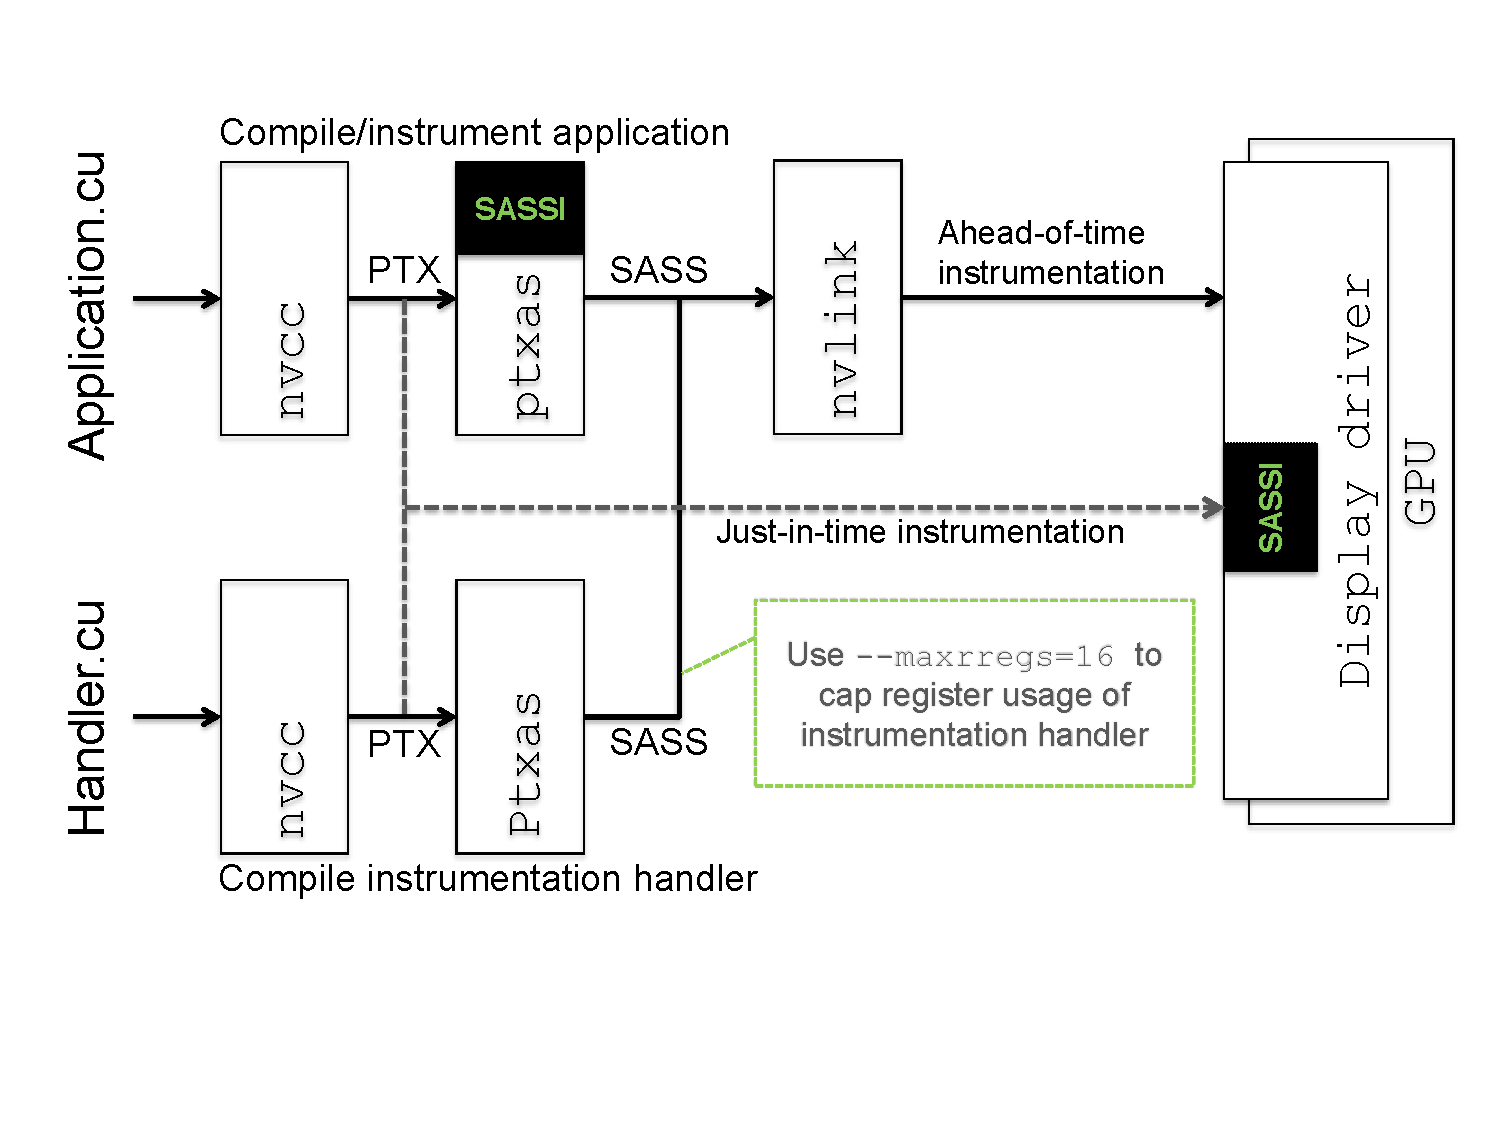
\includegraphics[width=0.60\textwidth]{figures/sassi-flow.pdf}
\caption{SASSI's instrumentation flow.}
\label{fig:sassi-comp-flow}
\end{figure}

Figure~\ref{fig:sassi-comp-flow} shows the compiler tool flow that
includes the SASSI instrumentation process.  Shaders are first
compiled to an intermediate representation by a \emph{front-end}
compiler.  Before they can run on the GPU, however, the \emph{backend}
compiler must read the intermediate representation and generate
SASS\@. When more than one module is compiled, the modules have to be
linked together using \texttt{nvlink} before running on the GPU.

SASSI is implemented as the final compiler pass in \texttt{ptxas}, and
as such it does not disrupt the perceived final instruction schedule
or register usage.  Furthermore as part of \texttt{ptxas}, SASSI is
capable of instrumenting programs written in languages that target
PTX, which includes CUDA and OpenCL.  Apart from the injected
instrumentation code, the original SASS code ordering remains
unaffected. With the SASSI prototype we use \texttt{nvlink} to link
the instrumented applications with user-level instrumentation
handlers.  SASSI could at some point in the future also be embedded in
the driver to JIT compile PTX inputs, as shown by dotted lines in
Figure~\ref{fig:sassi-comp-flow}.
